% =====================================================================
% 02_standards_spectrum.tex
% =====================================================================
\begingroup
\newcolumntype{L}[1]{>{\hsize=#1\hsize\raggedright\arraybackslash}X}
\newcolumntype{C}[1]{>{\hsize=#1\hsize\centering\arraybackslash}X}

\section{IEEE 802.11 Standards and Spectrum}
\label{sec:standards}

\subsection{Generations of Wi-Fi}

Table~\ref{tab:generations} summarises the main PHY amendments.
Generation names for 802.11b/a/g are informal and retroactive.

\begin{table}[htbp]
  \centering\footnotesize
  \caption{Wi-Fi generations and PHY amendments.}
  \label{tab:generations}
  \begin{tabularx}{\linewidth}{@{} L{1.1} C{0.4} C{0.6} C{0.5} C{0.4} C{0.8} L{2.2} @{}}
    \toprule
    \textbf{Generation / amendment} & \textbf{Year} & \textbf{Bands (GHz)} & \textbf{Max width (MHz)} & \textbf{Max QAM} & \textbf{Peak PHY rate} & \textbf{Key technologies}                                 \\
    \midrule
    -- / 802.11                     & 1997          & 2.4                  & 22                       & --               & 2~Mb/s                 & \acs{fhss}, \acs{dsss}, infrared; \acs{csmaca}            \\
    -- / 802.11b                    & 1999          & 2.4                  & 22                       & --               & 11~Mb/s                & HR-DSSS with \acs{cck}                                    \\
    -- / 802.11a                    & 1999          & 5                    & 20                       & 64               & 54~Mb/s                & \acs{ofdm} (52 subcarriers)                               \\
    -- / 802.11g                    & 2003          & 2.4                  & 20                       & 64               & 54~Mb/s                & \acs{ofdm} in 2.4~GHz, compatible with 11b                \\
    Wi-Fi~4 / 802.11n               & 2009          & 2.4, 5               & 40                       & 64               & 600~Mb/s               & \acs{mimo} (4 streams), channel bonding, \acs{ampdu}      \\
    Wi-Fi~5 / 802.11ac              & 2013          & 5                    & 160                      & 256              & 6.93~Gb/s              & 8 streams, downlink \acs{mumimo}, beamforming             \\
    Wi-Fi~6/6E / 802.11ax           & 2021          & 2.4, 5, 6            & 160                      & 1024             & 9.6~Gb/s               & \acs{ofdma}, UL/DL \acs{mumimo}, BSS Colouring, \acs{twt} \\
    Wi-Fi~7 / 802.11be              & 2024          & 2.4, 5, 6            & 320                      & 4096             & about 46~Gb/s          & \acs{mlo}, multi-\acs{ru}, preamble puncturing            \\
    \bottomrule
  \end{tabularx}
\end{table}

\subsection{Functional Amendments}

Besides PHY amendments, many amendments add MAC-level features. The
most relevant ones are listed in Table~\ref{tab:amendments}.

\begin{table}[htbp]
  \centering\footnotesize
  \caption{802.11 functional amendments.}
  \label{tab:amendments}
  \begin{tabularx}{\linewidth}{@{} L{0.5} L{0.9} L{1.6} @{}}
    \toprule
    \textbf{Amendment} & \textbf{Topic}             & \textbf{Purpose}                                            \\
    \midrule
    802.11e            & \acs{qos}                  & Prioritised channel access (\acs{edca}), basis of \acs{wmm} \\
    802.11h            & Spectrum management        & \acs{dfs} and \acs{tpc} for coexistence with radar in 5~GHz \\
    802.11i            & Security                   & \acs{ccmp}/\acs{aes}, 4-way handshake (WPA2)                \\
    802.11k            & Radio resource measurement & Neighbour reports and beacon measurements to assist roaming \\
    802.11r            & Fast BSS Transition        & Reduces handoff delay by pre-deriving keys                  \\
    802.11v            & \acs{btm}                  & Network can suggest a better \acs{ap} to a client           \\
    802.11w            & \acs{pmf}                  & Authenticates deauthentication/disassociation frames        \\
    802.11s            & Mesh networking            & Multi-hop forwarding between mesh \acp{ap}                  \\
    802.11u            & Interworking               & Basis of Passpoint/Hotspot~2.0 roaming agreements           \\
    802.11ai           & \acs{fils}                 & Fast initial authentication and link setup                  \\
    802.11ad / ay      & 60~GHz (DMG / EDMG)        & Short-range multi-gigabit links                             \\
    802.11ah           & Sub-1~GHz (Wi-Fi HaLow)    & Long-range, low-power \ac{iot}                              \\
    802.11az           & Positioning                & Improved ranging and location accuracy                      \\
    802.11ba           & Wake-up radio              & Ultra-low-power wake-up for \ac{iot} devices                \\
    802.11bf           & WLAN sensing               & Using Wi-Fi signals for presence and motion detection       \\
    \bottomrule
  \end{tabularx}
\end{table}

\subsection{Frequency Bands and Channels}

\subsubsection{The 2.4~GHz band}

Spanning roughly 2400--2483.5~MHz, the 2.4~GHz \ac{ism} band offers good range
and wall penetration but is narrow and crowded (Bluetooth, Zigbee, microwave
ovens, cordless phones). Channels are 5~MHz apart but a 20/22~MHz
signal overlaps about four adjacent channel numbers. Channels 1, 6 and 11 are
the usual non-overlapping planning choice. In Vietnam, the 2.4~GHz band
utilizes channels 1--13 and equipment must comply with the \ac{vnmic} technical
standards, such as \acs{qcvn} 54:2020/BTTTT, to determine permitted maximum
transmission power.

\begin{figure}[htbp]
  \centering
  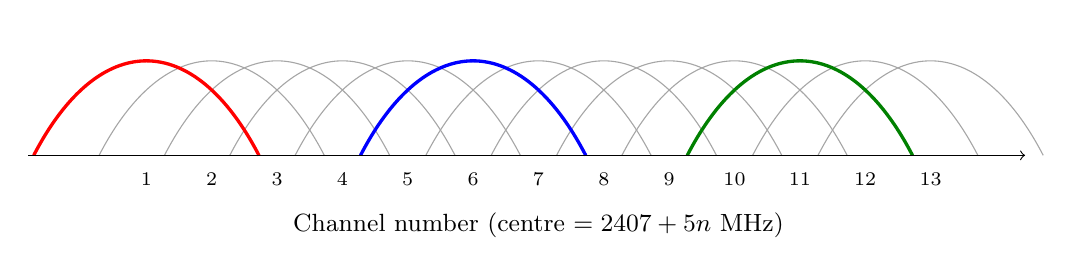
\begin{tikzpicture}
    \pgfmathsetmacro{\xscale}{0.83}
    \pgfmathsetmacro{\wband}{1.43}
    \pgfmathsetmacro{\wctrl}{0.6}
    \pgfmathsetmacro{\hpeak}{1.6}

    \foreach \n in
    {1,...,13}{
      \pgfmathsetmacro{\xc}{(\n - 1) * \xscale} \draw[gray!70] (\xc-\wband,0)
      .. controls (\xc-\wctrl,\hpeak) and (\xc+\wctrl,\hpeak) ..
      (\xc+\wband,0); \node[font=\scriptsize, anchor=north] at (\xc,-0.1)
      {\n};
    }
    \foreach \n/\col in
    {1/red, 6/blue, 11/green!50!black}{
      \pgfmathsetmacro{\xc}{(\n - 1) * \xscale} \draw[\col,very thick]
      (\xc-\wband,0) .. controls (\xc-\wctrl,\hpeak) and (\xc+\wctrl,\hpeak)
      .. (\xc+\wband,0);
    }
    \pgfmathsetmacro{\xend}{12 * \xscale + 1.2} \draw[->] (-1.5,0)
    -- (\xend,0);
    \node[font=\small, anchor=north] at ({6 * \xscale},-0.6)
    {Channel number (centre $= 2407 + 5n$~MHz)};
  \end{tikzpicture}
  \caption{2.4~GHz channel plan: channels 1, 6 and 11 (bold) do not overlap.}
  \label{fig:ch24}
\end{figure}

\subsubsection{The 5~GHz band}

The 5~GHz band is divided into sub-bands with different indoor, outdoor and
power conditions. Some channels require \ac{dfs}: an \ac{ap} must
listen for radar and vacate the channel if radar is detected. In
Vietnam, 5~GHz WLAN deployments are strictly regulated by the \acs{vnmic};
hardware must meet specific \acs{qcvn} standards for conformity certification
before clearing customs or deployment. The centre frequency of a 5~GHz
channel $n$ is
\begin{equation}
  f_c = 5000 + 5n \ \text{MHz}.
\end{equation}
Channels may be bonded into 40, 80 and 160~MHz widths, but wide channels reduce
the number of independent channels and increase the risk of co-channel interference.

\subsubsection{The 6~GHz band}

Wi-Fi~6E and Wi-Fi~7 can use the 6~GHz band. Under Vietnam's Circular
01/2025/TT-BKHCN (effective 15~May 2025), the 5925--6425~MHz spectrum is
officially allocated for Wi-Fi. Indoor usage is allowed up to 200~mW
\ac{eirp} (max \ac{psd} of 10~dBm/MHz), while outdoor deployments are limited to
25~mW \ac{eirp} (max \ac{psd} of 1~dBm/MHz). Devices are forbidden on
\acp{uas}. Where 6~GHz operation is permitted, WPA3 (or
\ac{owe}) is mandatory.

\subsubsection{Other bands}

The 60~GHz band (802.11ad/ay) offers very high rates over a few metres in a
single room. Sub-1~GHz (802.11ah, ``HaLow'') trades speed for range and
wall penetration for \ac{iot} sensors.

\subsection{Regulatory}

In Vietnam, the \ac{vnmic} sets national frequency allocation and technical
conformity (\acs{qcvn}) standards determining permitted WLAN channels, transmit
power, indoor and outdoor use, and \ac{dfs} requirements. Devices must
undergo mandatory conformity testing and obtain certification by
submitting a \ac{doc}.

\begin{tomtat}
\item Wi-Fi phát triển từ 802.11 (1997, 2~Mb/s) đến Wi-Fi~7 (802.11be: kênh 320~MHz, 4096-QAM, \acs{mlo}, tốc độ \acs{phy} lý thuyết tối đa khoảng 46~Gb/s). Tốc độ đỉnh chỉ là lý thuyết.
\item Các bản bổ sung chức năng cho \acs{phy}: \acs{qos} (e), \acs{dfs}/\acs{tpc} (h), bảo mật (i, w), chuyển vùng (k, r, v), mesh (s), cùng các bản cho \acs{iot}, định vị và cảm biến.
\item Băng 2,4~GHz: tầm xa, xuyên tường tốt nhưng hẹp và đông đúc; kênh 1, 6, 11 không chồng lấn; Việt Nam dùng kênh 1--13.
\item Băng 5~GHz: nhiều kênh hơn, có thể ghép 40/80/160~MHz, một số kênh yêu cầu \acs{dfs} để tránh radar.
\item Băng 6~GHz: theo Thông tư 01/2025/TT-BKHCN, dải 5925--6425~MHz dành cho Wi-Fi; trong nhà tối đa 200~mW \acs{eirp}, ngoài trời 25~mW, không được sử dụng trên \acs{uas}; bắt buộc WPA3 hoặc \acs{owe}.
\item Thiết bị tại Việt Nam phải tuân thủ các quy chuẩn \acs{qcvn} do \acs{vnmic} quy định, được kiểm tra hợp quy và nộp bản \acs{doc}.
\end{tomtat}
\endgroup
